Zur Erf�llung der Sonderaufgabe des Hardware-Aufbaus wurden folgende Teilleistungen erbracht:
\newline \\
Die Anbringung des UR5, PG70 und der Kinect Kamera wurden, wie in \ref{1-3-1_einleitung_systemarchitektur_hardware} beschrieben, erarbeitet und durchgef�hrt. Dabei wurde die Positionierung der Kinect Kamera so gew�hlt, dass sie zuz�glich des Tisches auch noch den Bereich neben dem UR5 einf�ngt. Welche Seite des Tisches vom Turtlebot angesteuert werden soll, wurde in Zusammenarbeit mit der zweiten Projektgruppe festgelegt.
\newline
Zusammen mit der dritten Gruppe wurde weiterhin entschieden, welche Tasse f�r die Live-Demo gegriffen werden soll. Dementsprechend wurde die maximale Griffbreite der Greiferfinger angepasst.
\newline
Die Modellierung der Szenerie als urdf-Modell \ref{urdfModell}, sowie das Aufsetzen der Simulation wurden ebenfalls im Zuge dieser Sonderaufgabe durchgef�hrt.
\begin{figure}
	\centering
	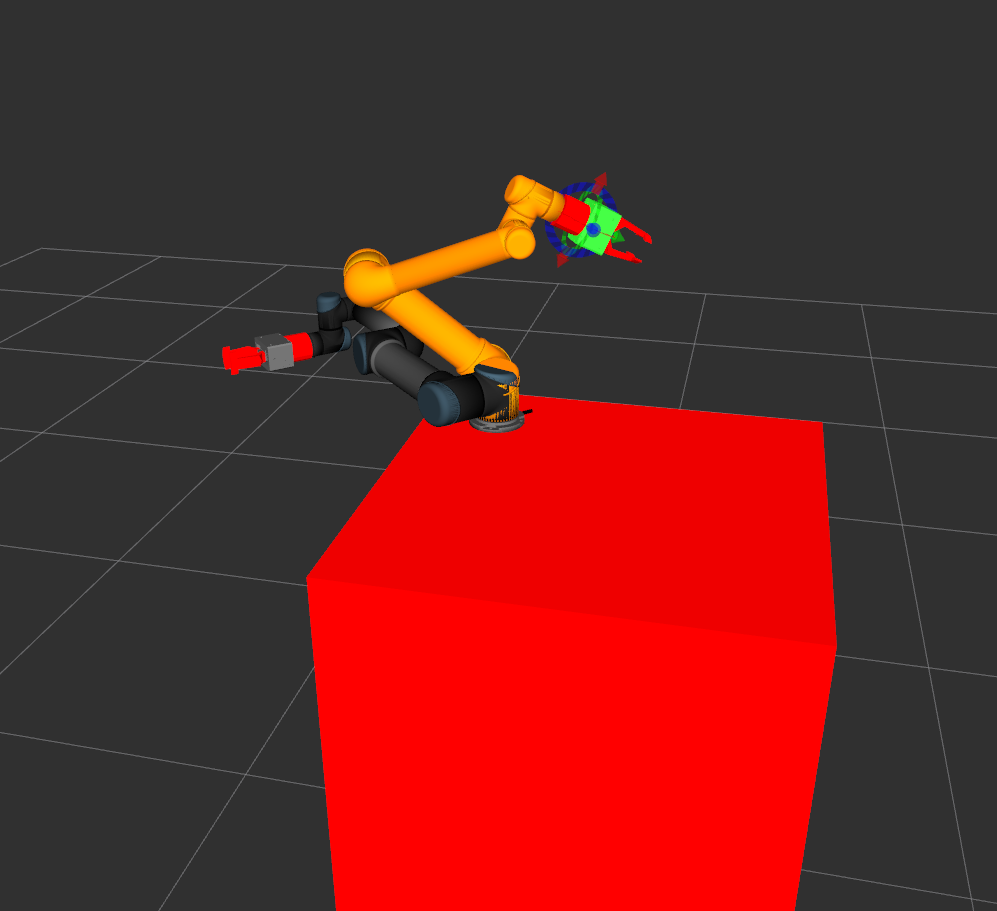
\includegraphics{images/Modell.png}
	\caption{Das f�r die Simulation und MoveIt-Bahnplanung verwendete urdf-Modell der statischen Szene.}
	\label{urdfModell}
\end{figure}